
Section~\ref{sec:background} described four families that all compress $t$
ephemeral secrets into one seed tree and then decide, per node, which seeds may
be released. We now isolate that mechanism, define the signature scheme built
on top of it, and state the invariant that the decision must satisfy.

\subsection{The seed-tree mechanism}

\begin{definition}[\GZKST]
\label{def:gzkst}
A \emph{Generic ZK Seed Tree} (\GZKST) is a tuple
$\Pi = (\Setup,\, \Expand,\, \Chal,\, \Decide,\, \Publish,\, \Recon)$
parametrised by a security parameter $\lam$, a number $t \in \mathbb{N}$ of
parallel repetitions, and a pseudorandom generator
$\PRG : \{0,1\}^{\lam} \to \{0,1\}^{2\lam}$. The six algorithms are:
\begin{enumerate}[leftmargin=*]
  \item $\Setup(1^{\lambda}) \to (\seed_r,\salt)$: samples a master seed
        $\seed_r \getsr \{0,1\}^{\lambda}$ and a public salt.

  \item $\Expand(\seed_r,\salt) \to (\calT,(\eseed_0,\ldots,\eseed_{t-1}))$:
        builds a binary tree $\calT$ by top-down \PRG-expansion from
        $\seed_r$, leaf $i$ holding $\eseed_i$. The topology may be complete
        or incomplete.

  \item $\Chal(\cmt_0,\ldots,\cmt_{t-1},\msg) \to
        \mathbf{c} = (c_0,\ldots,c_{t-1})$: derives a fixed-weight
        Fiat--Shamir challenge from the round commitments and the message.

  \item $\Decide(\mathbf{c}) \to (\calH,\calR)$: partitions
        $\{0,\ldots,t-1\}$ into the hidden set $\calH = \{i : c_i \neq 0\}$,
        $|\calH| = w$, and the revealed set $\calR = \{i : c_i = 0\}$.

  \item $\Publish(\calT,\calH) \to \tpath$: returns a set of nodes from which
        every $\eseed_i$ with $i \in \calR$ is reconstructible and no
        $\eseed_i$ with $i \in \calH$ is derivable.

  \item $\Recon(\tpath,\mathbf{c},\salt) \to \{\eseed_i : i \in \calR\}$:
        verifier-side reconstruction of the revealed leaf seeds.
\end{enumerate}
\end{definition}

Definition~\ref{def:gzkst} describes only the seed machinery; it says nothing
about secrets or messages. To speak about key recovery we must say how a
signature scheme is built on top of it, which is the content of the next
definition.

\subsection{The derived signature scheme}
\label{sec:derived}

\begin{definition}[Round functions]
\label{def:round}
A \emph{round system} for a \GZKST\ $\Pi$ over a secret type $\calS$ (the type
of the long-term secret: monomial permutations for LESS, matrix pairs for
MEDS, an R-SDP solution for CROSS, a witness for MPCitH) is a triple
$(\Commit, \Resp, \ChkRnd)$ of efficient algorithms:
\begin{itemize}[leftmargin=*]
  \item $\Commit(\eseed_i, \salt, i) \to \cmt_i$: derives the round-$i$
        ephemeral secret from the leaf seed and commits to it. It does not
        take $\sk$.
  \item $\Resp(\eseed_i, c_i, \sk) \to \resp_i$: for a hidden round, combines
        the ephemeral secret with the component of $\sk \in \calS$ selected by
        $c_i$.
  \item $\ChkRnd(\resp_i, c_i, \pk, i) \to \cmt_i$ or $\perp$: recomputes the
        round-$i$ commitment from the response alone, without $\eseed_i$.
\end{itemize}
\end{definition}

\begin{definition}[Derived signature scheme]
\label{def:sigma}
Given $\Pi$ and a round system as above, the \emph{derived signature scheme}
$\Sig[\Pi]$ is the pair $(\Sign, \Verify)$ of Algorithm~\ref{alg:generic}.
\end{definition}

\begin{figure}[htbp]
\centering
\begin{minipage}[t]{0.48\textwidth}
\begin{algorithm}[H]
\small
\setlength{\algomargin}{0.9em}
\caption{$\Sig[\Pi].\Sign$}
\label{alg:generic}
\KwIn{Secret key $\sk$, message $\msg$}
\KwOut{Signature $\sig$}
$(\seed_r,\salt) \leftarrow \Setup(1^{\lam})$\;
$(\calT,(\eseed_i)_i) \leftarrow \Expand(\seed_r,\salt)$\;
\lFor{$i = 0$ \KwTo $t-1$}{$\cmt_i \leftarrow \Commit(\eseed_i,\salt,i)$}
$\mathbf{c} \leftarrow \Chal(\cmt_0,\ldots,\cmt_{t-1},\msg)$\;
$(\calH,\calR) \leftarrow \Decide(\mathbf{c})$\;
\lFor{$i \in \calH$}{$\resp_i \leftarrow \Resp(\eseed_i,c_i,\sk)$}
$\tpath \leftarrow \Publish(\calT,\calH)$\;
\Return $\sig \leftarrow \bigl(\mathbf{c},(\resp_i)_{i\in\calH},\tpath,\salt\bigr)$
\end{algorithm}
\end{minipage}\hfill
\begin{minipage}[t]{0.48\textwidth}
\begin{algorithm}[H]
\small
\setlength{\algomargin}{0.9em}
\caption{$\Sig[\Pi].\Verify$}
\label{alg:generic-verify}
\KwIn{Public key $\pk$, message $\msg$, signature $\sig$}
\KwOut{$\mathsf{accept}$ or $\perp$}
Parse $\sig$ as $(\mathbf{c},(\resp_i)_{i\in\calH},\tpath,\salt)$\;
$(\calH,\calR) \leftarrow \Decide(\mathbf{c})$\;
$\{\eseed_i\}_{i \in \calR} \leftarrow \Recon(\tpath,\mathbf{c},\salt)$\;
\lFor{$i \in \calR$}{$\widehat{\cmt}_i \leftarrow \Commit(\eseed_i,\salt,i)$}
\lFor{$i \in \calH$}{$\widehat{\cmt}_i \leftarrow \ChkRnd(\resp_i,c_i,\pk,i)$}
\lIf{some $\widehat{\cmt}_i = \perp$}{\Return $\perp$}
\lIf{$\Chal(\widehat{\cmt}_0,\ldots,\widehat{\cmt}_{t-1},\msg) = \mathbf{c}$}
   {\Return $\mathsf{accept}$}
\Return $\perp$
\end{algorithm}
\end{minipage}
\end{figure}

\begin{remark}
MEDS instantiates Definition~\ref{def:round} by setting
\[
  \Commit(\sigma_i,\alpha,i) \;=\;
  \Compress\bigl(\SF(\pimap{\tilde{A}_i}{\tilde{B}_i}(G_0))\bigr),
\]
with $\Resp$ given by~\eqref{eq:meds-resp}, and with $\ChkRnd$ applying
$(\mu_i,\nu_i)$ to $G_{h_i}$. Comparing Algorithm~\ref{alg:generic} with
Algorithm~\ref{alg:sign_meds} line by line makes the correspondence explicit:
the digest $d$ plays the role of $\mathbf{c}$, and line~16 is $\Publish$.
\end{remark}
% ------------------------------------------------------------
\textbf{The Flag Structure.}
The flag structure $\calF$ produced internally by $\Publish$ is the key
intermediate object.  It is a labelling $\calF : V(\calT) \to \{0,1\}$ where:
\begin{itemize}
  \item $\calF(v) = 0$: node $v$ is \emph{publishable}---either
        directly included in $\tpath$ or derivable from a published ancestor;
  \item $\calF(v) = 1$: node $v$ is \emph{hidden}---it must not appear in $\tpath$ and must not be derivable from published nodes.
\end{itemize}
The flag structure satisfies two invariants:

Throughout we use the convention $\calF(\mathsf{parent}(\mathrm{root})) = 1$,
so that the root itself may belong to $\tpath$.

\begin{invariant}[Correctness]
\label{inv:correctness}
For every $i \in \calR$ there exists a node $v$ on the path from the root to
leaf $\eseed_i$ such that $\calF(v) = 0$ and $\calF(\mathsf{parent}(v)) = 1$.
\end{invariant}

\begin{invariant}[ZK hiding]
\label{inv:hiding}
For every $i \in \calH$, no ancestor of leaf $\eseed_i$ satisfies $\calF(v) = 0$.
\end{invariant}

The ZK property of the signature scheme is contingent on
Invariant~\ref{inv:hiding} holding for \emph{all} $i \in \calH$. A fault that
changes $\calF(v)$ from $1$ to $0$ for any $v$ that is an ancestor of some
$\eseed_i$ with $i \in \calH$ \emph{breaks Invariant~\ref{inv:hiding}} and
may allow an attacker to reconstruct $\eseed_i$. We provide an example of
the GGM tree, together with the concepts of the hidden tree and flag
structure, in Figure~\ref{fig:less-trees}.


\subsection{Mapping Schemes to the GZKST Model}
\label{sec:mapping}

We now establish that the MEDS signature scheme
introduced in Section~\ref{sec:background}, as well as two other zero-knowledge-base 
postquantum signature schemes, LESS-v2~\cite{LESS-spec} and CROSS~\cite{CROSSspec}, are 
valid \GZKST\ instances in the
sense of Definition~\ref{def:gzkst}.  We exhibit the concrete
instantiation of the six algorithms and verify that
Invariants~\ref{inv:correctness} and~\ref{inv:hiding} hold by construction.


\begin{proposition}[MEDS is a \GZKST\ instance]
\label{prop:meds-gzkst}
MEDS instantiates Definition~\ref{def:gzkst} with secret type
$\calS = \{(A_j^{-1}, B_j^{-1})\}_{j=1}^{s-1}$,
$t$ parallel repetitions, and a \GGM\ tree of height
$\lceil \log_2 t \rceil$ (complete when $t$ is a power of two,
incomplete otherwise; only the first $t$ of the $2^{\lceil\log_2 t\rceil}$
leaves are used).
Invariants~\ref{inv:correctness} and~\ref{inv:hiding} hold by the
$\SeedTreeToPath$ construction regardless of whether the tree is
complete or incomplete; see Appendix~\ref{app:proof-meds}.
\end{proposition}

The six algorithms instantiate as follows. $\Setup$ derives $(\seed_r,\salt)$
from a single $\XOF$ call, and $\Expand$ builds the height-$\lceil\log_2 t\rceil$
tree by hashing each parent with the salt and node index, returning the first
$t$ leaves (the rightmost $2^{\lceil\log_2 t\rceil}-t$ are unused when $t$ is not
a power of two). $\Chal$ expands each leaf into ephemeral
matrices, hashes the compressed generators with $m$, and parses the digest via
$\ParseHash_{s,t,w}$ into $\mathbf{h}\in\{0,\ldots,s-1\}^t$ of weight $w$;
$\Decide$ then sets $\calH=\{i:h_i\neq0\}$, $\calR=\{i:h_i=0\}$. Finally,
$\Publish=\SeedTreeToPath_t$ applies the bottom-up rule
$\calF(v)=\calF(\ell)\vee\calF(r)$ and serialises the boundary nodes
(Invariant~\ref{inv:correctness}) in depth-first order, while
$\Recon=\PathToSeedTree_t$ re-expands them downward, leaving the positions
$i\in\calH$ empty.

\begin{remark}
  This $\Publish$ description follows the MEDS submission~\cite{MEDS_PQC}; the
  reference implementation uses a different algorithm, detailed in
  Section~\ref{sec:app}.
\end{remark}


The same instantiation extends to LESS-v2 and CROSS, yielding
Propositions~\ref{prop:less-gzkst} and~\ref{prop:cross-gzkst}; the proofs
follow the MEDS argument (Appendix~\ref{app:proof-meds}).

\begin{proposition}[LESS-v2 is a \GZKST\ instance]
\label{prop:less-gzkst}
LESS-v2\cite{LESS-spec} instantiates Definition~\ref{def:gzkst} with secret type
$\calS = \{\pi_1, \ldots, \pi_{s-1}\}$ (the $s-1$ secret monomial permutations),
$t$ parallel repetitions, and an \emph{incomplete} \GGM\ tree of height
$\lceil \log_2 t \rceil$.
Invariants~\ref{inv:correctness} and~\ref{inv:hiding} hold by construction
of the three-phase flag tree.
\end{proposition}

\begin{remark}[Invariants under incomplete trees]
\label{rem:incomplete}
When the tree is incomplete, some leaves appear at depth
$\lceil \log_2 t \rceil - 1$. The LESS-v2 index-tracking arrays
keep $\LabelLeaves$ and $\ComputeSeeds$ on the correct nodes regardless of
level, so both invariants hold for any tree shape the expansion produces.
\end{remark}

\begin{figure}[tb]
\centering
\begin{minipage}[b]{0.42\linewidth}
\centering
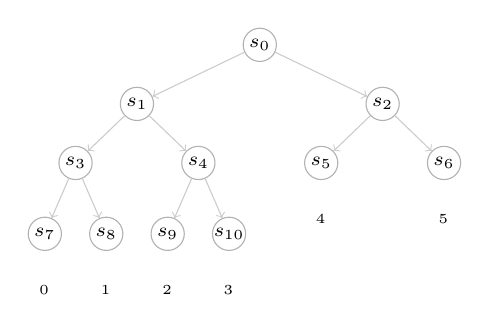
\begin{tikzpicture}[x=0.78cm, y=1.0cm]
  \tikzstyle{neutnode}  = [circle, draw=gray!60, fill=white, text=black, minimum size=12pt, inner sep=0pt, font=\scriptsize]
  \tikzstyle{treeedge} = [gray!40, rounded corners=2pt,->, thin]
  \tikzstyle{leaflbl}  = [font=\tiny, below=1pt]
  \node[neutnode](s0) at (3.5,0){$s_0$};
  \node[neutnode](s1) at (1.5,-.75){$s_1$};
  \node[neutnode](s2) at (5.5,-.75){$s_2$};
  \node[neutnode](s3) at (.5,-1.5){$s_3$};
  \node[neutnode](s4) at (2.5,-1.5){$s_4$};
  \node[neutnode](s5) at (4.5,-1.5){$s_5$};
  \node[neutnode](s6) at (6.5,-1.5){$s_6$};
  \node[neutnode](s7) at (0,-2.4){$s_7$};
  \node[neutnode](s8) at (1,-2.4){$s_8$};
  \node[neutnode](s9) at (2,-2.4){$s_9$};
  \node[neutnode](s10) at (3,-2.4){$s_{10}$};
  \node[leaflbl] at (0,-2.9){$\eseed_0$};
  \node[leaflbl] at (1,-2.9){$\eseed_1$};
  \node[leaflbl] at (2,-2.9){$\eseed_2$};
  \node[leaflbl] at (3,-2.9){$\eseed_3$};
  \node[leaflbl] at (4.5,-2.0){$\eseed_4$};
  \node[leaflbl] at (6.5,-2.0){$\eseed_5$};
  \draw[treeedge](s0)--(s1);\draw[treeedge](s0)--(s2);
  \draw[treeedge](s1)--(s3);\draw[treeedge](s1)--(s4);
  \draw[treeedge](s2)--(s5);\draw[treeedge](s2)--(s6);
  \draw[treeedge](s3)--(s7);\draw[treeedge](s3)--(s8);
  \draw[treeedge](s4)--(s9);\draw[treeedge](s4)--(s10);
  
\end{tikzpicture}
\vspace{2pt}
{\small (a) Expanded reference \GGM\ seed tree.}
\end{minipage}%
\hfill%
\begin{minipage}[b]{0.55\linewidth}
\centering
\begin{tikzpicture}[x=0.78cm, y=1.0cm]
  \tikzstyle{neutnode} = [circle, draw=gray!60, fill=nodehid, text=black, minimum size=12pt, inner sep=0pt, font=\scriptsize]
  \tikzstyle{pubnode}  = [circle, draw=green!50!black, fill=nodepath, minimum size=12pt, inner sep=0pt, font=\scriptsize]
  \tikzstyle{zeronode} = [circle, draw=gray!60, fill=nodepub, minimum size=12pt, inner sep=0pt, font=\scriptsize]
  \tikzstyle{treeedge} = [gray!40, rounded corners=2pt,->, thin]
  \tikzstyle{leaflbl}  = [font=\tiny, below=1pt]
  \node[neutnode](s0) at (3.5,0){$s_0$};
  \node[neutnode](s1) at (1.5,-.75){$s_1$};
  \node[neutnode](s2) at (5.5,-.75){$s_2$};
  \node[neutnode](s3) at (.5,-1.5){$s_3$};
  \node[pubnode] (s4) at (2.5,-1.5){$s_4$};
  \node[neutnode](s5) at (4.5,-1.5){$s_5$};
  \node[pubnode] (s6) at (6.5,-1.5){$s_6$};
  \node[pubnode] (s7) at (0,-2.4){$s_7$};
  \node[neutnode](s8) at (1,-2.4){$s_8$};
  \node[zeronode](s9) at (2,-2.4){$s_9$};
  \node[zeronode](s10) at (3,-2.4){$s_{10}$};
  \node[leaflbl] at (0,-2.9){$\eseed_0$};
  \node[leaflbl] at (1,-2.9){$\eseed_1$};
  \node[leaflbl] at (2,-2.9){$\eseed_2$};
  \node[leaflbl] at (3,-2.9){$\eseed_3$};
  \node[leaflbl] at (4.5,-2.0){$\eseed_4$};
  \node[leaflbl] at (6.5,-2.0){$\eseed_5$};
  \draw[treeedge](s0)--(s1);\draw[treeedge](s0)--(s2);
  \draw[treeedge](s1)--(s3);\draw[treeedge](s1)--(s4);
  \draw[treeedge](s2)--(s5);\draw[treeedge](s2)--(s6);
  \draw[treeedge](s3)--(s7);\draw[treeedge](s3)--(s8);
  \draw[treeedge](s4)--(s9);\draw[treeedge](s4)--(s10);
  
\end{tikzpicture}
\vspace{2pt}
{\small (b) After \Chal, \Decide, \Publish; $\mathbf{b}\!=\!\{0,1,0,0,1,0\}$, $\tpath\!=\!\{s_4,s_6,s_7\}$.}
\end{minipage}
\caption{GGM seed tree ($t=6$): structure~(a) and flag state~(b).
In~(b): pink nodes ($\calF{=}1$, hidden subtree); green nodes ($\calF{=}0$,
fully revealed subtree); blue-bordered nodes ($\calF{=}0$, in $\tpath$).}
\label{fig:less-trees}
\end{figure}

\begin{comment}
\begin{itemize}
    \item $\Setup(1^{\lam}) \to (\seed_r, \salt)$: The root seed is derived from the secret key seed; the salt is sampled uniformly at random.
    \item $\Expand(\seed_r, \salt) \to (\calT, (\eseed_0, \ldots, \eseed_{t-1}))$:
LESS-v2 uses an incomplete \GGM\ tree with $\lceil \log_2 t \rceil$ levels.
Leaves are distributed across the bottom two levels; index offsets are
tracked via $\mathsf{npl}$, $\mathsf{ll}$, $\mathsf{off}$, and $\mathsf{lsi}$
(Figure~\ref{fig:less-trees}a).
    \item $\Chal(\cmt, \msg) \to \mathbf{c}$:
The $t$ canonical-form matrices together with the salt and message are
hashed; $\SampleChallenge$ produces
$\mathbf{b} \in \{0,\ldots,s-1\}^t$ of weight $w$.
Setting $c_i = b^{(i)}$, the condition $c_i = 0$ (resp.\ $c_i \neq 0$)
signals a revealed (resp.\ hidden) round.
    \item $\Decide(\mathbf{c}) \to (\calH, \calR)$:
$\calH = \mathrm{supp}(\mathbf{b})$, $\calR = \{0,\ldots,t-1\} \setminus \calH$.
    \item $\Publish(\calT, \calH) \to \tpath$:
LESS-v2 builds an auxiliary flag tree of the same shape via two phases:
(i)~\emph{leaf labelling} ($\LabelLeaves$):
$\calF(\mathrm{leaf}_i) = \mathbf{1}[i \in \calH]$;
(ii)~\emph{upward propagation} ($\ComputeSeeds$): $\calF(v) = \calF(\ell) \vee \calF(r)$
for each internal node $v$ with children $\ell$ and $r$.
The two-phase description is an implementation detail; the resulting flag
assignment is exactly the OR-propagation of equations~\eqref{eq:leaf-flag}--\eqref{eq:or-prop}
(the root's flag is determined solely by this propagation).
The path $\tpath = \{v : \calF(v) = 0,\; \calF(\mathrm{parent}(v)) = 1\}$
(with the convention that $\calF(\mathrm{parent}(\mathrm{root})) = 1$)
is the minimal publishable boundary (Figure~\ref{fig:less-trees}b).
    \item $\Recon(\tpath, \mathbf{c}, \salt) \to \{\eseed_i : i \in \calR\}$:
$\PathToSeedTree$ places received nodes on an empty tree of the same shape
and re-expands downward via $\PRG$ until all $t$ leaves are filled.
Positions $i \in \calH$ remain empty; positions $i \in \calR$ yield the
recovered seeds from which monomial matrices and commitments are re-derived.
\end{itemize}
\end{comment}



\begin{proposition}[CROSS is a \GZKST\ instance]
\label{prop:cross-gzkst}
CROSS~\cite{CROSSspec} instantiates Definition~\ref{def:gzkst} with secret type
$\calS = \{\mathbf{e}\}$ (the R-SDP solution),
$t$ parallel repetitions, and a complete \GGM\ tree.
The seed-publishing component satisfies
Invariants~\ref{inv:correctness} and~\ref{inv:hiding} by the same argument
as MEDS (Proposition~\ref{prop:meds-gzkst}).
The additional Merkle proof over $\{\mathsf{cmt}_0[i]\}_{i \in \calH}$ is
a CROSS-specific commitment-authenticity mechanism orthogonal to the
\GZKST\ seed-hiding invariants.
\end{proposition}


 
\begin{comment}
\begin{itemize}
    \item $\Setup(1^{\lam}) \to (\seed_r, \salt)$: Root seed of size $\lam$ bits and salt of size $2\lam$ bits, both drawn uniformly at random.
    \item $\Expand(\seed_r, \salt) \to (\calT, (\eseed_0, \ldots, \eseed_{t-1}))$:
A complete binary tree (CROSS-v1 identical to LESS-v1; CROSS-v2 uses the
$\SeedTreePath$ mechanism of MEDS) where each parent seed is concatenated
with the salt and node index and processed by SHAKE to yield two $\lam$-bit child seeds.
    \item $\Chal(\cmt, \msg) \to \mathbf{c}$:
CROSS applies Fiat--Shamir in two rounds.
The $t$ commitment pairs $(\mathsf{cmt}_0[i], \mathsf{cmt}_1[i])$, the salt,
and the message are hashed to produce $\mathsf{chall}_1 \in (\mathbb{F}_p^*)^t$,
from which first-response digests $y_i = \mathrm{Hash}(\mathbf{u}'_i + \mathsf{chall}_1[i] \cdot \mathbf{e}'_i)$ are derived.
A second hash yields $\mathsf{chall}_2 \in \mathcal{B}(t,w)$; setting
$c_i = \mathsf{chall}_2[i] \in \{0,1\}$, $c_i = 0$ (resp.\ $1$) signals
a revealed (resp.\ hidden) round.
    \item $\Decide(\mathbf{c}) \to (\calH, \calR)$:
$\calH = \{i : c_i = 1\}$, $\calR = \{i : c_i = 0\}$.
    \item $\Publish(\calT, \calH) \to \tpath$:
The seed path is computed as in MEDS.  Additionally, a Merkle proof over
$\{\mathsf{cmt}_0[i]\}_{i \in \calH}$ authenticates the $w$ commitment values
that the verifier cannot recompute; this is orthogonal to the \GZKST\
seed-hiding invariants (see Proposition~\ref{prop:cross-gzkst}).
    \item $\Recon(\tpath, \mathbf{c}, \salt) \to \{\eseed_i : i \in \calR\}$:
Path nodes are placed on an empty tree and re-expanded downward.
Positions $i \in \calH$ remain empty; positions $i \in \calR$ yield seeds
from which $({\bf e}'_i, {\bf u}'_i)$ are re-derived and $\mathsf{cmt}_1[i]$
is recomputed for verification.
\end{itemize}


\begin{definition}[Faulted Signing Oracle]
\label{def:fault-oracle}
Fix a node $v^* \in V(\calT)$.
The \emph{faulted signing oracle} $\Oracle^{v^*}(\sk, \pk)$ takes a
message $\msg$ and executes the signing algorithm with a single
modification: during $\Publish(\calT, \calH)$, the flag value is
forced to
\[
  \calF(v^*) \;\leftarrow\; 0,
\]
regardless of whether $\calF(v^*)$ equals $1$ in the honest execution.
Upward propagation is applied as normal after this assignment.
The oracle returns the resulting (possibly faulted) signature $\sig^*$.
\end{definition}
\end{comment}

\subsection{Oracle Abstraction}
\label{sec:oracle}

To model fault attacks, we extend the \GZKST abstraction with a faulted signing oracle and a secret-extraction procedure.

\begin{definition}[Faulted Signing Oracle]
\label{def:fault-oracle}
Let $\Pi=(\Setup,\Expand,\Chal,\Decide,\allowbreak
\Publish,\allowbreak\Recon)$ be a \GZKST
instance, let $\Sig[\Pi]$ be the derived signature scheme of
Definition~\ref{def:sigma}, and let $(\sk,\pk)$ be a fixed key pair. For a
node $v^*\in V(\calT)$, the oracle $\Oracle^{v^*}(\sk,\pk)$ runs
$\Sig[\Pi].\Sign(\sk,\msg)$ unmodified except that, during
$\Publish(\calT,\calH)$, it forces
$\calF(v^*) \leftarrow 0$
before the normal upward propagation step. The oracle outputs the
resulting (possibly faulted) signature $\sig^*$.
\end{definition}

A fault is \emph{effective} if $v^*$ originally satisfies
$\calF(v^*)=1$ and is an ancestor of some hidden leaf
$\eseed_i$ with $i\in\calH$. In this case, the published path
reveals a node from which $\eseed_i$ is derivable, violating
Invariant~\ref{inv:hiding}. Otherwise, the fault is
\emph{ineffective}.

\begin{remark}
Definition~\ref{def:fault-oracle} captures several practical fault
mechanisms, including instruction skips, stuck-at-zero faults,
bit-flips, and clock glitches~\cite{ZKFault,FaultToForge2025}.
\end{remark}

\begin{remark}
We assume access to an algorithm \texttt{SolverS} that efficiently
recovers secrets of type $\calS$ once sufficient information is
revealed. For LESS, for example, this follows from
Lemma~1 of~\cite{ZKFault}.
\end{remark}

For every hidden round $i\in\calH$, a valid signature reveals the
response $\resp_i$ while keeping $\eseed_i$ hidden. An effective
fault breaks this separation: the attacker obtains both
$\resp_i$ and $\eseed_i$. We call this event
\emph{dual revelation}; it is the basic primitive underlying all
secret-recovery attacks considered in this work.



\begin{comment}
\subsection{Oracle Abstraction}
\label{sec:oracle}

We previously presented the abstract view of the \GGM-tree and its
instantiations in LESS, MEDS, and CROSS.
We now formalize the attacker's interface in an abstract manner,
extending the \GZKST tuple with a fault model and a secret-extraction
procedure.


\noindent\textbf{Faulted signing oracle.}
Let $\Pi = (\Setup,\Expand,\Chal,\Decide,\Publish,\Recon)$ be a
\GZKST\ instance with secret type $\calS$, and let
$(\sk, \pk)$ be a fixed key pair.
We model the adversary's access to the victim's signing device as a
\emph{faulted oracle}:

\begin{definition}[Faulted Signing Oracle]
\label{def:fault-oracle}
Fix a node $v^* \in V(\calT)$.
The \emph{faulted signing oracle} $\Oracle^{v^*}(\sk, \pk)$ takes a
message $\msg$ and executes the signing algorithm with a single
modification: during $\Publish(\calT, \calH)$, the flag value is
forced to
\[
  \calF(v^*) \;\leftarrow\; 0,
\]
regardless of whether $\calF(v^*)$ equals $1$ in the honest execution.
Upward propagation is applied as normal after this assignment.
The oracle returns the resulting (possibly faulted) signature $\sig^*$.
\end{definition}

\noindent
The fault is \emph{effective} if the original value $\calF(v^*)$ was
$1$ and $v^*$ is an ancestor of at least one leaf $\eseed_i$ with
$i \in \calH$: in this case, the published path $\tpath$ now contains
a node from which $\eseed_i$ is derivable, directly violating
Invariant~\ref{inv:hiding}.
The fault is \emph{ineffective} otherwise (the node was already
publishable, or all hidden leaves lie in the sibling subtree).

\begin{remark}
The fault model of Definition~\ref{def:fault-oracle} is realised by
several concrete physical mechanisms: an instruction-skip fault that
bypasses the store $\calF(v) \leftarrow \calF(\ell) \vee \calF(r)$,
a stuck-at-zero perturbation forcing $\calF(v^*)=0$, a bit-flip
$(1 \to 0)$ via Rowhammer, or a clock-glitch that skips the validity
check on a specific tree node.  All of these are documented in the
literature~\cite{ZKFault,FaultToForge2025}.
\end{remark}

\begin{remark}
  We assume that our faulted oracle has an algorithm \texttt{SolverS}
  that efficiently solves secrets of type $\calS$. For example, when
  instantiating our oracle against LESS, we use Lemma~1 from~\cite{ZKFault}
  to solve the secret type.
\end{remark}

\noindent\textbf{Dual revelation.}
The invariant that the $\Publish$ phase must enforce is that, for
every hidden round $i \in \calH$, the signer simultaneously publishes:
\begin{itemize}
  \item[(i)] the ZK \emph{response} $\resp_i$, which encodes the
             relationship between $\eseed_i$ and the long-term secret
             $\sk$; and
  \item[(ii)] a path $\tpath$ from which $\eseed_i$ is
              \emph{not} derivable.
\end{itemize}
An effective fault breaks condition~(ii): the attacker now holds both
$\eseed_i$ (reachable from the faulted path) and $\resp_i$ (always
present in the signature).  This \emph{dual revelation} is the
primitive from which all secret-extraction procedures in this work
are built.
\end{comment}

\begin{comment}
\begin{figure}[tb]
\centering
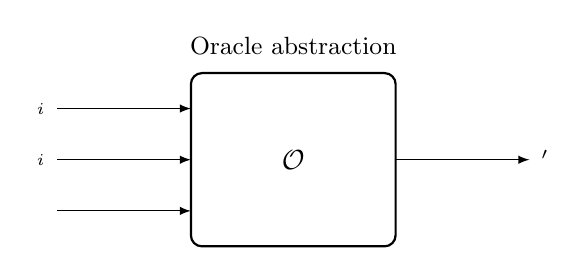
\begin{tikzpicture}[>=latex, x=1cm, y=1cm]
% Oracle box
\draw[rounded corners=4pt, line width=0.8pt] (-1.3,-1.1) rectangle (1.3,1.1);
\node at (0,0) {$\mathcal{O}$};
\node[font=\small] at (0, 1.45) {Oracle abstraction};
% Input labels
\node[font=\small] (s)   at (-3.2,  0.65) {$\eseed_i$};
\node[font=\small] (r)   at (-3.2,  0.00) {$\resp_i$};
\node[font=\small] (pk)  at (-3.2, -0.65) {$\pk$};
% Output label
\node[font=\small] (out) at ( 3.2,  0.00) {$\sk'$};
% Arrows
\draw[->] (-3.0,  0.65) -- (-1.3,  0.65);
\draw[->] (-3.0,  0.00) -- (-1.3,  0.00);
\draw[->] (-3.0, -0.65) -- (-1.3, -0.65);
\draw[->] ( 1.3,  0.00) -- ( 3.0,  0.00);
\end{tikzpicture}
\caption{The \Extract\ oracle: given dual revelation $(\eseed_i, \resp_i)$
and public key $\mathsf{pk}$, it outputs partial secret $\mathsf{sk}'$.}
\label{fig:oracle}
\end{figure}
\end{comment}


\subsection{A taxonomy of fault surfaces}
\label{sec:taxonomy}

The value of Definitions~\ref{def:gzkst} and~\ref{def:sigma} is not that they
restate the (obvious) fact that revealing a hidden seed breaks zero knowledge.
It is that they make the fault surface \emph{enumerable}. Every implementation
of $\Sig[\Pi]$ must materialise each of the components in turn, and each
component admits its own class of faults with its own consequence:

\begin{itemize}[leftmargin=*]
  \item $\Setup$: biasing or zeroing $\seed_r$ makes the whole tree
        predictable, and hence every $\eseed_i$, without touching $\Publish$
        at all.
  \item $\Expand$: skipping a \PRG\ invocation leaves a child node at a
        known or stale value. This is the surface exploited against
        FAEST~\cite{JendralD25} and against Mirath/RYDE~\cite{BandaBK26}.
  \item $\Chal$: corrupting the digest before it is parsed changes which
        rounds are hidden.~\cite{HuangHHYSTY26} skips iterations
        of the digest-preprocessing loop of LESS-v2 and never touch the tree.
  \item $\Decide$: forcing $c_i \leftarrow 0$ for some $i$ moves a round from
        $\calH$ to $\calR$, so the seed is published \emph{legitimately} while
        $\resp_i$ has already been emitted.
  \item $\Publish$: corrupting the per-node release decision. This is the
        surface of ZKFault~\cite{ZKFault}, of
        Fault-to-Forge~\cite{FaultToForge2025}, and of all three attacks in
        Section~\ref{sec:app}.
  \item $\Recon$: verifier-side, and therefore relevant to signature
        acceptance rather than key recovery; we note it for completeness and
        return to it in Section~\ref{sec:counter}, since a
        verify-before-release countermeasure runs $\Recon$ on the signer's own
        device.
\end{itemize}

Table~\ref{tab:surfaces} places the published attacks on this grid. Two
observations follow. First, five independent attacks that were developed
against four different schemes, with different tree shapes and different
secret types, land on only three of the six components --- which is evidence
that the grid is the right coordinate system rather than an artefact.
Second, the empty cells are predictions, and one of them is what led us to
Model~2 of Section~\ref{sec:app}: asking ``what \emph{else} inside $\Publish$
can be faulted, besides the flag value itself?'' points at the index
bookkeeping that walks the tree, a surface with no analogue in the LESS flag
array and one that no previous work had considered.

\begin{table}[htbp]
\centering
\caption{Published fault attacks on \GZKST-based signatures, classified by the
component of Definitions~\ref{def:gzkst}--\ref{def:round} that the fault
corrupts.}
\label{tab:surfaces}
\small
\setlength{\tabcolsep}{4pt}
\begin{tabular}{@{}lccccc@{}}
\toprule
 & \textbf{LESS} & \textbf{MEDS} & \textbf{CROSS}
 & \textbf{\begin{tabular}[c]{@{}c@{}}RYDE/\\ Mirath\end{tabular}}
 & \textbf{FAEST} \\ \midrule
\textbf{\begin{tabular}[c]{@{}l@{}}ZKFault\\~\cite{ZKFault}\end{tabular}}
  & \Publish & \Publish
  & \begin{tabular}[c]{@{}c@{}}\Publish\\ (not tested)\end{tabular} & -- & -- \\ \addlinespace
\textbf{\begin{tabular}[c]{@{}l@{}}Fault to Forge\\~\cite{FaultToForge2025}\end{tabular}}
  & \Publish & -- & -- & -- & -- \\ \addlinespace
\textbf{\begin{tabular}[c]{@{}l@{}}Faultless Key Recovery\\~\cite{HuangHHYSTY26}\end{tabular}}
  & \Chal & -- & -- & -- & -- \\ \addlinespace
\textbf{\begin{tabular}[c]{@{}l@{}}Fault Attack on MPCitH\\~\cite{BandaBK26}\end{tabular}}
  & -- & -- & -- & \begin{tabular}[c]{@{}c@{}}\Expand,\\ \Chal\end{tabular} & -- \\ \addlinespace
\textbf{\begin{tabular}[c]{@{}l@{}}Case Study on FAEST\\~\cite{JendralD25}\end{tabular}}
  & -- & -- & -- & -- & \Expand \\ \addlinespace
\midrule
\textbf{This work (Section~\ref{sec:app})}
  & -- & \begin{tabular}[c]{@{}c@{}}\Publish\\ ($3$ surfaces)\end{tabular}
  & -- & -- & -- \\
\bottomrule
\end{tabular}
\end{table}

\begin{remark}[Specification versus implementation]
\label{rem:spec-vs-impl}
A single scheme may realise the same component in two inequivalent ways. The
MEDS specification~\cite{MEDS_PQC} describes $\Publish$ as the bottom-up
OR-propagation $\calF(v) = \calF(\ell) \vee \calF(r)$ followed by a
depth-first serialisation of the boundary; the reference implementation
instead performs a depth-first descent driven by an index cursor into the
sorted list of hidden leaves, with no flag array at all. Both satisfy
Invariants~\ref{inv:correctness} and~\ref{inv:hiding}, so both are correct,
but they have disjoint fault surfaces. Analysing the abstraction alone is
therefore not sufficient, and analysing one implementation does not transfer
to another; Section~\ref{sec:app} attacks the implementation.
\end{remark}

\subsection{Secret extraction and key recovery}

Extraction is the inverse of $\Resp$ once the leaf seed is known:

\begin{definition}[Extract]
\label{def:extract}
$\Extract(\eseed_i, \resp_i, \pk) \to \sk'$: given the leaked seed
$\eseed_i$ and the ZK response $\resp_i$ for the same round $i \in \calH$,
recover the (partial) secret $\sk' \subseteq \calS$.
\end{definition}

Equivalently, $\Extract$ inverts $\Resp$ once its first argument is known.
For the schemes studied in this work it is instantiated as follows.
\begin{itemize}
  \item \textbf{MEDS}.
        For a hidden round $i$ with $h_i = j$, the signer publishes
        $(\mu_i, \nu_i) = (\widetilde{A}_iA_j^{-1},\, B_j^{-1}\widetilde{B}_i)$
        (consistent with the background description in \S\ref{sec:meds}).
        Expanding $\eseed_i$ yields $(\widetilde{A}_i, \widetilde{B}_i)$,
        so
        \[
          A_j^{-1} \;=\; \widetilde{A}_i^{-1} \cdot \mu_i ,
          \qquad
          B_j^{-1} \;=\; \nu_i \cdot \widetilde{B}_i^{-1}.
        \]
        Both operations are direct matrix multiplications and inversions
        over $\mathbb{F}_q$; no column-reconstruction step is required.
  \item \textbf{LESS-v2}.
        The response is a coset representative
        $\CosetRep(\pi_{b[i]} \circ \tilde{\pi}_i^*)$.
        Expanding $\eseed_i$ gives the partial monomial matrix
        $\tilde{\pi}_i^*$, and the secret permutation $\pi_{b[i]}$ is
        recovered via the column-extraction argument of
        Lemma~1 in~\cite{FaultToForge2025}.
  \item \textbf{CROSS}.
        The response encodes $\mathbf{v}_i = \mathbf{e} \star
        (\mathbf{e}'_i)^{-1}$.
        Expanding $\eseed_i$ gives $\mathbf{e}'_i$, so
        $\mathbf{e} = \mathbf{v}_i \star \mathbf{e}'_i$ directly.
\end{itemize}

\noindent\textbf{Full key recovery.}
When $|\calS| = s - 1 > 1$ (as in MEDS with $s \geq 3$, and
LESS with $s \geq 3$), a single effective fault recovers only the secret
indexed by $h_i$.  Full recovery requires observing each index
$j \in \{1,\ldots,s-1\}$ at least once.

\begin{algorithm}[tb]
\caption{GZKST key recovery from faulted oracle}
\label{alg:key-recovery}
\SetKwInOut{Input}{Input}
\SetKwInOut{Output}{Output}
\Input{Faulted oracle $\Oracle^{v^*}$, public key $\pk$}
\Output{Recovered secret key $\widehat{\sk}$}
$\mathsf{Collected} \leftarrow \emptyset$\;
\While{$|\mathsf{Collected}| < |\calS|$}{
  $\sig^* \leftarrow \Oracle^{v^*}(\msg)$ for an arbitrary $\msg$\;
  \If{$\sig^*$ is \emph{effective}}{
    \For{each $i \in \mathsf{leaked}(\sig^*)$}{
      $\sk' \leftarrow \Extract\!\left(\eseed_i,\, \resp_i,\, \pk\right)$\;
      $\mathsf{Collected} \leftarrow \mathsf{Collected} \cup \{(j, \sk')\}$
        where $j = c_i$\;
    }
  }
}
\Return $\widehat{\sk} \leftarrow \mathsf{Collected}$\;
\end{algorithm}

\begin{proposition}[Correctness of Algorithm~\ref{alg:key-recovery}]
\label{prop:alg-correctness}
Let $\Pi$ be a \GZKST\ instance, suppose $v^* = \mathrm{root}$
(so the fault exposes all $w$ hidden leaves, making $L = w$ deterministic),
and let $p_{\min} = 1 - \bigl(\tfrac{s-2}{s-1}\bigr)^{\!w}$.
Algorithm~\ref{alg:key-recovery} terminates and outputs $\widehat{\sk} = \sk$
with probability at least $1 - \delta$ after at most
$\left\lceil \dfrac{s-1}{p_{\min}} \cdot \ln\!\dfrac{1}{\delta} \right\rceil$
effective oracle queries; see Appendix~\ref{app:proof-recovery} for the full proof.
\end{proposition}

\begin{remark}[General fault location]
\label{rem:general-fault}
For an effective fault at an arbitrary node $v^*$ with $\ell$ leaf
descendants, the number $L = |\calH \cap \mathrm{leaves}(v^*)|$ of hidden
leaves in the subtree is a hypergeometric random variable whose realisation
may be smaller than its mean $\bar{w} = w\ell/t$, making the per-query
success probability $p_r(L) = 1-\bigl((s{-}1{-}r)/(s{-}1)\bigr)^{\!L}$
potentially smaller than the root-fault $p_{\min}$.  A valid bound for any
effective fault is obtained by taking the worst case $L = 1$, which gives
$p_r \geq r/(s-1)$ for all $r \geq 1$ and therefore
$\mathbb{E}[Q] \leq (s-1)\,H_{s-1}$,
where $H_{s-1} = \sum_{r=1}^{s-1}1/r$ is the $(s{-}1)$-th harmonic number.
For $s \leq 6$ (all schemes in Table~\ref{tab:scheme-params}), this gives
$\mathbb{E}[Q] \leq 5H_5 \approx 11.4$, still a small constant.
\end{remark}

\noindent
Detecting whether a received signature is effective is feasible for
the adversary: given the fault location $v^*$ and the challenge $\mathbf{c}$
(recoverable from the digest $d$ in the signature), the adversary recomputes
the honest flag tree, checks whether $\calF(v^*) = 1$, and verifies that at
least one hidden leaf falls in the subtree of $v^*$.
This detection is detailed for LESS in~\cite{ZKFault} and applies
unchanged to MEDS and CROSS.

\noindent\textbf{Expected query count.}
With $p_{\min}$ as in Proposition~\ref{prop:alg-correctness}, the root fault
admits a clean expectation bound.

\begin{proposition}
\label{prop:query-count}
Let $v^* = \mathrm{root}$, so $L = w$ exactly. Then $p_r \geq p_{\min}$ for all
$r \geq 1$, and the expected total number of effective queries satisfies
$\mathbb{E}[Q] \leq (s-1)/p_{\min}$.
See Appendix~\ref{app:proof-query} for the derivation.
\end{proposition}

\begin{remark}[Role of Jensen's inequality]
\label{rem:edist}
The per-query gain $E_{\mathrm{dist}} = (s-1)\,p_{\min}$ is the expected number
of distinct secret indices revealed when $L = w$ is deterministic at the root.
For $v^* \neq \mathrm{root}$, convexity of $\alpha^x$ makes $E_{\mathrm{dist}}$
an \emph{upper} bound on per-query gain, hence only a \emph{lower} bound on
$\mathbb{E}[Q]$; the bound in Proposition~\ref{prop:query-count} relies solely
on the direct inequality $p_r \geq p_{\min}$, not on the Jensen argument.
\end{remark}

Table~\ref{tab:meds-eq} instantiates the root-fault bound
($p_{\min} = 1 - ((s-2)/(s-1))^w$, $L = w$ exactly) for every MEDS parameter
set: since $\ell = t$ gives $\bar{w} = w \gg 1$, all sets have
$p_{\min} > 0.99$ and $\mathbb{E}[Q] \leq s-1 \leq 5$.

\begin{table}[h]
\centering
\caption{Expected effective queries $\mathbb{E}[Q]$ for MEDS (fault at root).}
\label{tab:meds-eq}
\begin{tabular}{@{}lrrrrr@{}}
\toprule
Parameter set & $s$ & $w$ & $s{-}1$ & $p_{\min}$ & $\mathbb{E}[Q] \leq$ \\
\midrule
MEDS-9923   & 4 &  14 & 3 & 0.9966 & 3.01 \\
MEDS-13220  & 5 &  20 & 4 & 0.9968 & 4.01 \\
MEDS-41711  & 4 &  26 & 3 & 1.0000 & 3.00 \\
MEDS-69497  & 5 &  36 & 4 & 1.0000 & 4.00 \\
MEDS-134180 & 5 &  52 & 4 & 1.0000 & 4.00 \\
MEDS-167717 & 6 &  66 & 5 & 1.0000 & 5.00 \\
\bottomrule
\end{tabular}
\end{table}

\noindent\textbf{From key recovery to forgery.}
Once Algorithm~\ref{alg:key-recovery} terminates, the adversary holds
a complete signing key $\widehat{\sk}$ and can produce valid signatures
on any message $\msg^*$ — including messages never submitted to any
oracle.  This constitutes a full break of EUF-CMA:

\begin{corollary}
\label{cor:euf-cma}
Let $\Pi$ be a \GZKST-based signature scheme and let the fault model be as in
Definition~\ref{def:fault-oracle} (a stuck-at-zero perturbation of a single
flag bit during $\Publish$).  If an efficient adversary can induce this fault
at a fixed node $v^* \in V(\calT)$ on the victim's signing device, then
$\Pi$ is \emph{not} \textrm{EUF-CMA}-secure in the fault model: the adversary
recovers $\sk$ via Algorithm~\ref{alg:key-recovery} and forges signatures on
arbitrary messages without further oracle access.
\end{corollary}
